\documentclass[a4paper,12pt]{article}

\usepackage[utf8]{inputenc}
\usepackage{amsmath}
\usepackage{graphicx}
\usepackage{hyperref}
\usepackage{geometry}
\usepackage[labelfont=bf]{caption}
\usepackage{caption}
\usepackage{subcaption}
\usepackage{indentfirst}
\usepackage{placeins}
\usepackage{listings}

\setlength\parindent{24pt}

\geometry{a4paper, margin=1in}
\setlength{\parindent}{24pt}
\begin{document}

\begin{titlepage}
    \centering
    {\large\bfseries RANCANG BANGUN SISTEM TRANSAKSI TIKET PESAWAT BERBASIS APLIKASI DESKTOP GUI DENGAN BAHASA C DAN DATABASE MYSQL\par}
    \vspace{0.3cm}
    {\large\bfseries PROJECT AKHIR\par}
    {\large\bfseries PRAKTIKUM DASAR PEMROGRAMAN\par}
    \vspace{2cm}
    \vspace*{0.5cm}
    
\includegraphics[width=0.4\textwidth]{Logo_PENS.png}\par\vspace{1cm}
    \vspace{1cm}
    {\large\bfseries Dosen :\par}
    {\Large Norma Ningsih, S.ST., M.T.\par}
    \vspace{1cm}
    {\large\bfseries Oleh :\par}
    {\Large Muqsith Barru Pamungkas - 2423600035\\Riski Gana Prasetya - 2423600053\par}
    \vspace{1cm}
    {\scshape\LARGE Teknologi Rekayasa Internet \par}
    {\scshape\LARGE Departemen Teknik Elektro \par}
    \vspace{0.5cm}
    {\scshape\Large POLITEKNIK ELEKTRONIKA NEGERI SURABAYA\par}
    {\scshape\Large 2024\par}
    \vfill
\end{titlepage}

\section{Tujuan}
\label{sec:intro}

\begin{itemize}
    \item  Merancang sistem penjualan dan pembelian tiket pesawat menggunakan bahasa C berbasis GUI (GTK) dengan MySQL sebagai database
\end{itemize}

\section{Pendahuluan}
\subsection{Latar Belakang}
Sistem Pembelian dan Penjualan Tiket Pesawat "Myber" yang dibuat ini merupakan sebuah sistem transaksi/e-commerce berbasis aplikasi desktop (GUI) yang dibuat dengan menggunakan bahasa C dan GTK atau GIMP Toolkit sebagai framework untuk membangun tampilan, serta mengintegrasikan sebuah database menggunakan MySQL.

Sistem yang dirancang memiliki dua fungsi utama yaitu untuk penjualan dan pembelian tiket pesawat. Sehingga aplikasi ini memiliki dua tipe pengguna, yaitu admin sebagai penjual dan memiliki akses untuk membuat atau mengupdate detail tiket yang dijual, lalu
terdapat pengguna atau customer yang berada di sisi pembeli. Dari sisi pengguna atau customer sendiri dapat melakukan register atau pendaftaran akun.

Dalam pengembangan aplikasi ini, kami melakukan development di lingkungan/environment Linux, menggunakan distro Ubuntu 22.04.4 LTS WSL (kernel 5.15.146.1-microsoft-standard-WSL2) dan Arch Linux (kernel: 6.9.3-zen1-1-zen). Kami menggunakan Makefile (make) untuk melakukan otomasi dalam men-compile kode dengan gcc.


\subsection{Bahasa C}
Bahasa C oleh Dennis M. Ritchie pada tahun 1972 di laboratorium Bell ditemukan. Pengembangan BPCL (Basic Combined Program Language) yang dibuat oleh Dr.
Martin Richard yang selanjutnya dikembangkan oleh Ken Thompson dan diseleksi dengan
Language B.Dari ketertarikan Dennis pada penerjemah bahasa B, kemudian dikembangkan menjadi
sebuah kompiler yang disebut C.
Bahasa pemrograman C merupakan sebuah bahasa pemrograman tingkat menengah yang relatif mudah untuk di pelajari, sekain bahasa yang mudah untuk di pelajari bahasa c juga memiliki kemampuan performa yang tinggi serta
bahasa c mempunyai sifat portable dalam hal ini bahasa c yang ditulis dalam satu komputer bisa dipindahkan ke komputer lain tanpa mengotak-atiknya,tanpa muncul kerumitan dalam modifikasinya. 
Dalam pengaplikasiannya bahasa C sering digunakan dalam pembuatan berbagai aplikasi seperti sistem operasi,antivirus,hingga compiler bahasa pemrograman, bahasa c ini juga merupakan induk dari beberapa bahasa seperti bahasa C++, C-Sharp, dan java.
Karena sifat bahasa c yang mudah dipahami, bahasa c menjadi bahasa pemrograman yang paling sering digunkan.
% tambahi maneh kurang okeh ketoke 

\subsection{GIMP Toolkit (GTK)}
GUI atau singkatan dari Graphical User Interface yang memungkinkan pengguna untuk berinteraksi dengan perangkat keras komputer serta memudahkan dalam mengoperasikan sebuah sistem operasi (user friendly). GUI adalah sarana 
penghubug antara si pengguna(user) dengan aplikasi yang digunakan. Salah satu jenis Toolkit GUI yang populer adalah GIMP Toolkit atau GTK. 
GTK atau dikenal juga GIMP ToolKit adalah software yang digunakan untuk membangun sebuah tampilan aplikasi(GUI) lintas platform yang pertama kali dikembangkan oleh
GNU Image Manipulation Program (GIMP). ToolKit ini menyediakan berbagai macam widget yang sangat membantu dalam pembuatan aplikasi dan mampu support langsung berbagai bahasa seperti c,c++,dan pythpon
% ini juga tambahi neh seh kurang

\subsection{MySQL}
MySQL, yang dibaca MY-ES-KYOO-EL, adalah sebuah sistem manajemen database relasional (RDBMS) yang bersifat open source dan dibangun berdasarkan Bahasa Pertanyaan Struktural (SQL). Dengan kata lain, MySQL adalah sebuah program yang menggunakan bahasa pemrograman SQL untuk membuat dan mengelola berbagai jenis data yang ada pada database di server. Tiga orang Swedia bernama David Axmark, Allan Larsson, dan Michael Widenius adalah pendiri MySQL, yang dikembangkan pada tahun 1994 oleh perusahaan asal Swedia bernama MySQL AB. Pada tanggal 23 Mei 1995, versi stabil pertama MySQL muncul setelah kurang lebih satu tahun pengembangan.

Pada tahun 2008, Sun Microsystems membeli hak milik MySQL dari Oracle, raksasa teknologi Amerika. Singkatnya, Oracle memiliki hak cipta MySQL. MySQL saat ini adalah salah satu pilihan database yang paling populer untuk berbagai tujuan, seperti membuat dan mengelola database, penyimpanan data, mengelola transaksi e-commerce, pencatatan data, dan, yang paling umum, sebagai database untuk website.

% otw
\section{Instalasi dan Tampilan Aplikasi}
% Berikut ini tampilan dari aplikasi yang kami buat
\subsection{Pra-instalasi dan kompilasi}
Berikut ini package-package yang dibutuhkan sebelum melakukan kompilasi :
\begin{itemize}
    \item \texttt{gcc} untuk instalasi gcc (GNU Compiler Collection).
    \item \texttt{libgtk-3-dev} untuk instalasi GTK-3.
    \item \texttt{mysql-server} untuk instalasi MySQL server.
    \item \texttt{default-libmysqlclient-dev} untuk client library C MySQL.
    \item \texttt{build-essential} (opsional) untuk instalasi paket gcc sekaligus make di Ubuntu, merupakan meta-package yang berisi berbagai package yang berguna untuk mengcompile program.
\end{itemize}

\subsection{Proses Kompilasi}
Dalam melakukan kompilasi, pastikan semua package yang dibutuhkan telah terinstal, selanjunya adalah melakukan kompilasi dengan menggunakan make.

Makefile merupakan sebuah file yang berisi sekumpulan perintah atau set yang dapat digunakan menggunakan make untuk melakukan otomatisasi agar mencapai tujuan tertentu, dalam hal ini yaitu melakukan kompilasi.
Berikut ini isi dari Makefile yang kami buat untuk mempermudah proses kompilasi.
\begin{figure}[!htbp]
    \centering
    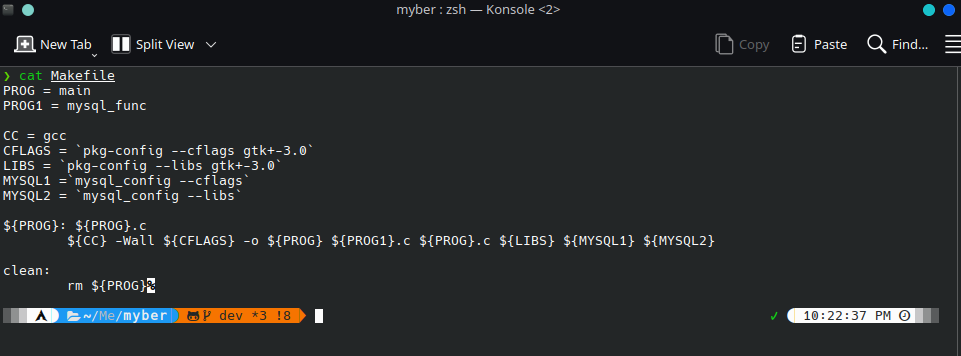
\includegraphics[width=1\textwidth]{./Makefile.png}
    \caption{Makefile}

\end{figure}
\FloatBarrier 

Selanjutnya untuk melakukan kompilasi, gunakan perintah berikut :

\begin{lstlisting}[language=bash]
make
\end{lstlisting}

\begin{figure}[!htbp]
    \centering
    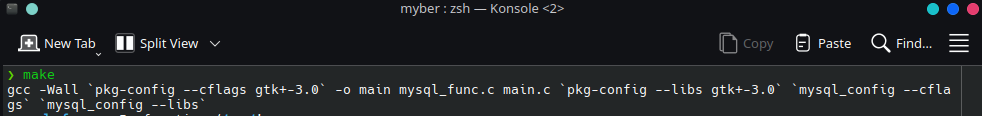
\includegraphics[width=1\textwidth]{./Make.png}
    \caption{Make}

\end{figure}
\FloatBarrier

Selanjutnya file binary program akan dihasilkan dari proses kompilasi, untuk menjalankan gunakan perintah :

\begin{lstlisting}[language=bash]
    ./main
\end{lstlisting}

\begin{figure}[!htbp]
    \centering
    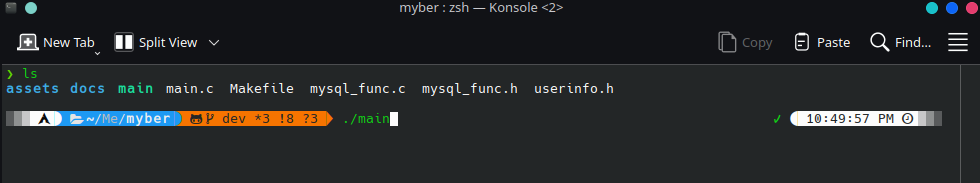
\includegraphics[width=1\textwidth]{./Main.png}
    \caption{File program hasil kompilasi}

\end{figure}
\FloatBarrier 

\subsection{Welcome Screen}
Berikut ini adalah tampilan ketika aplikasi pertama kali dibuka

\begin{figure}[!htbp]
    \centering
    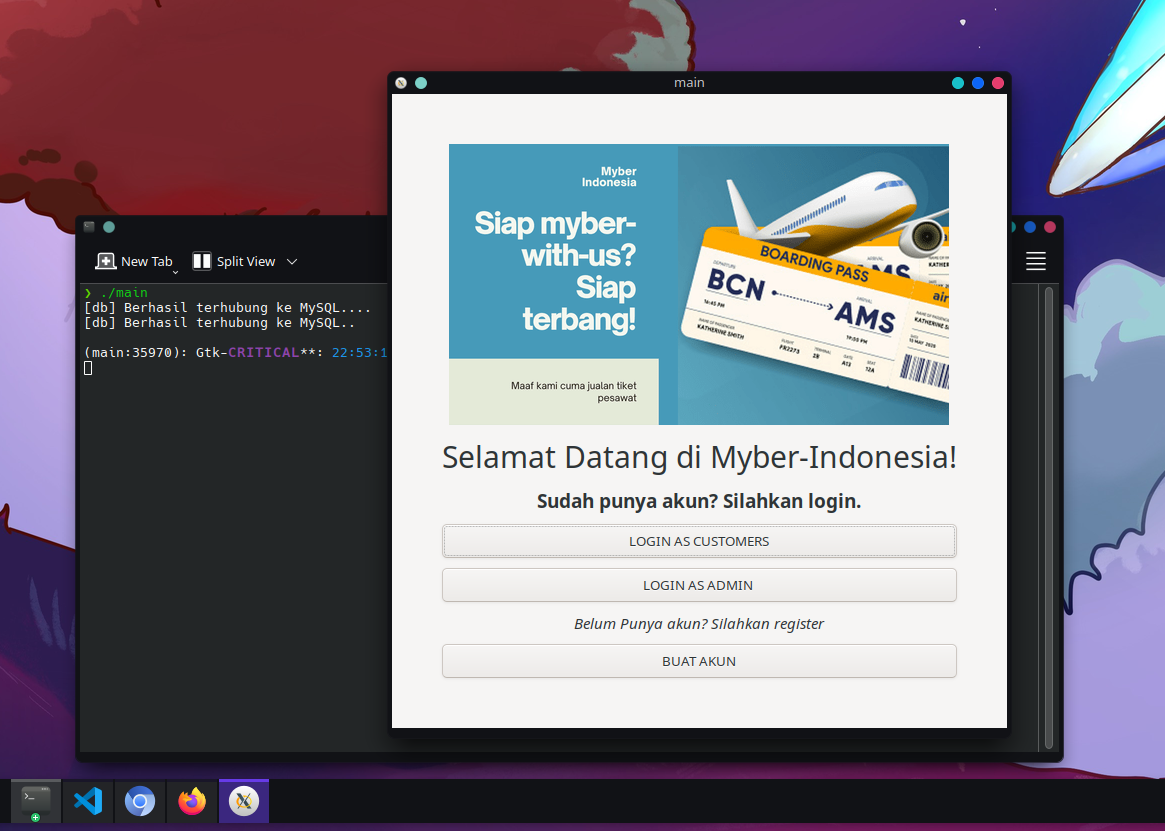
\includegraphics[width=1\textwidth]{./Welcome.png}
    \caption{File program hasil kompilasi}

\end{figure}
\FloatBarrier 

\subsection{Customer - Halaman Register}
Berikut merupakan tampilan halaman register untuk pengguna/customer
\begin{figure}[!htbp]
    \centering
    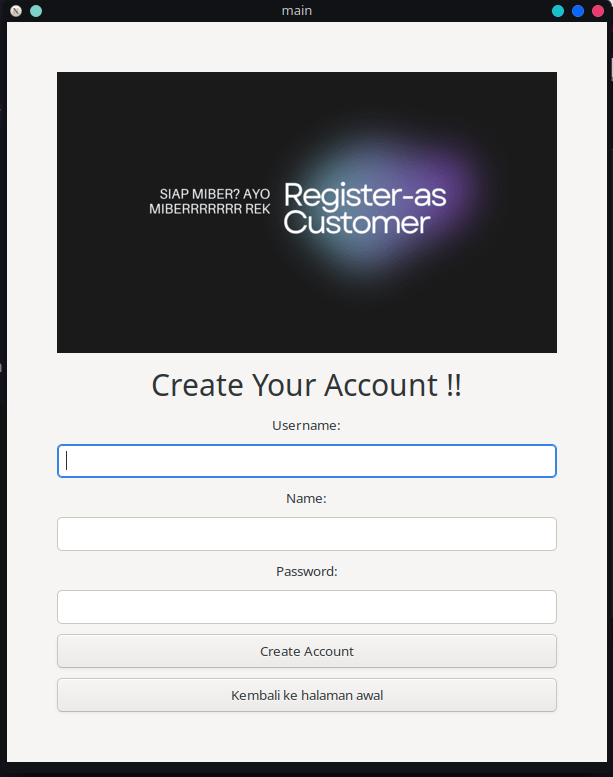
\includegraphics[width=0.43\textwidth]{./Register.png}
    \caption{Halaman Register Customer}

\end{figure}
\FloatBarrier 

\subsection{Customer - Halaman Login}
Ini merupakan tampilan halaman login untuk pengguna/customer
\begin{figure}[!htbp]
    \centering
    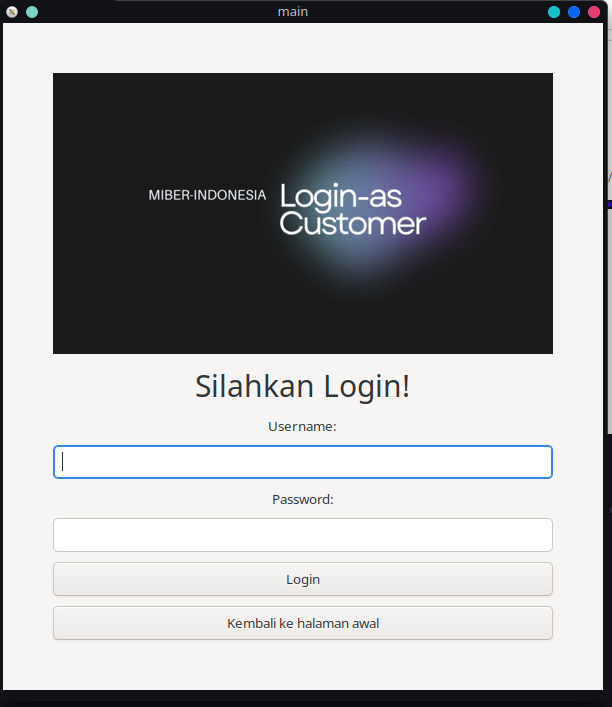
\includegraphics[width=0.43\textwidth]{./Login.png}
    \caption{Halaman Login Customer}

\end{figure}
\FloatBarrier 

\subsection{Admin - Halaman Login}
Selanjutnya adalah halaman login admin, dengan tampilan sebagai berikut:
\begin{figure}[!htbp]
    \centering
    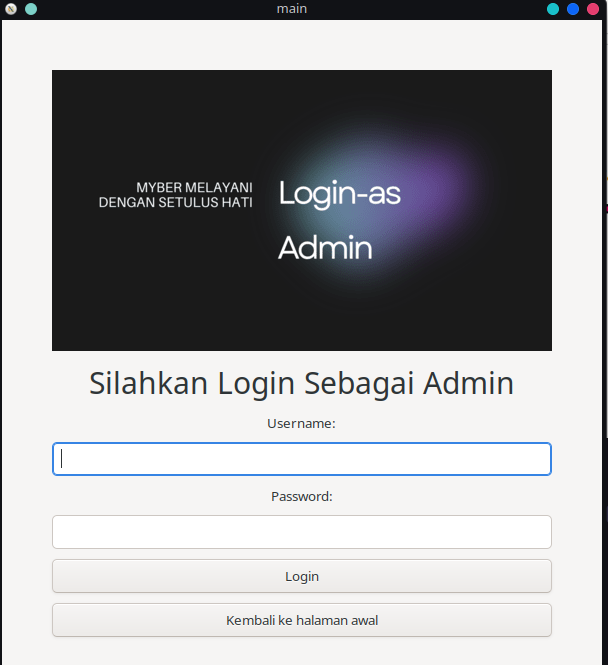
\includegraphics[width=0.43\textwidth]{./Login_admin.png}
    \caption{Halaman Login Admin}

\end{figure}
\FloatBarrier 

\section{Kode Program}
Kode program dari aplikasi kami lampirkan dalam folder, dan juga pada repository github berikut :
\begin{itemize}
    \item \url{https://github.com/indonumberone/myber}
\end{itemize}

\section{Analisa}

\section{Kesimpulan}

\end{document}
